\chapter{Work Object}%
\label{ch:workobject}
\markboth{Work Object}{}

\begin{flushright}
	{\smaller
		\textit{Citazione\\ citazione}\\
		-- Autore}
\end{flushright}

\section {Introduction}
In JPAD it is possible to read an .XML file as input or generate an object whose data are written in the code. Both in the first and in the second case all needed variables are initialized with data relating the choosen aircraft. The difference between these two methos is that using an .XML file, user can to define its own aircraft having clear view about the needed data useful for the analysis.\\
Contrariwise in order to perform test of program functionality, to use a default aircraft is the most simple way to generate a work object.

\section {Input data from .XML file}
%\subsection{XML File Format}
XML is a file extension for an {\itshape Extensible Markup Language (XML)} file format used to create common information formats and share both the format and the data on the World Wide Web, intranets, and elsewhere using standard ASCII text.
It is defined ``Markup Language'' due to the use of tags that describes the content. XML is considered extensible because the markup symbols are unlimited and self-defining. So it is possible to use personal tag for each data. In this way to read an .XML file results relatively simple .\\
The key concepts of an .XML File Format are the followings:
\begin{itemize}
\item markup symbol (tag)
\item attribute
\item tree structure
\end{itemize}

As mentioned, each part of the test is contained between an opening {\bfseries markup symbol} and an end markup symbol that expressed the meaning of the text.\\

\begin{figure}[H]
\centering
{
\includegraphics[height=0.31cm]{Immagini/xml1.jpg}} 
\caption{Use of markup symbols in XML language.}
\end{figure}

In addition to tag name, the markup symbols may contain also some {\bfseries attributes} that introduce more informations such as the unit of measure.\\

\begin{figure}[H]
\centering
{
\includegraphics[height=0.4cm]{Immagini/xml2.jpg}} 
\caption{Use of attributes in XML language.}
\end{figure}

An .XML file has a tree structure where there are extenal knots that branch into internal knots.
%\noindent \\
%
%\begin{figure}[H]
%\centering
%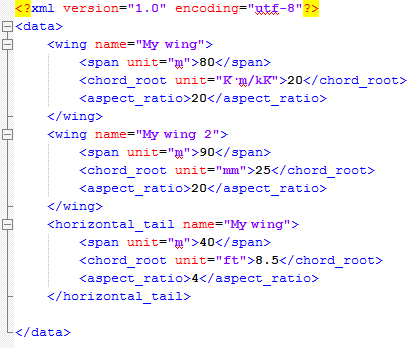
\includegraphics[height=6cm]{Immagini/xml5.png}\hfil
%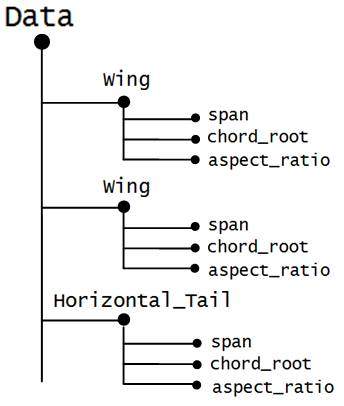
\includegraphics[height=6cm]{Immagini/xml3.jpg}
%\caption{Tree structure of an .XML file.}
%\end{figure}

%\subsection{Data Managment from XML file.}
In order to read an XML file it is necessary, first of all, to give the file path. The class \texttt{JPADXmlReader} opens the file and  the methods of the class \texttt{MyXMLReaderUtils} reads the useful data from the XML having the tag path as input. It is possible to read data as \texttt{Amount}, namely with units of measurement or as \texttt{double}. The unit of measurement is written in the attributes of data in XML file.\\ 

Likewise it is possible to write output data on XML file using \texttt{JPADDataWriter} class. First of all it is necessary to define and build the xml tree structure. After each variable is associated to a name that is the markup symbol of the XML file.

%possibili sviluppi futuri

\section {Default Aircraft}
Actually it is possible to define two different aircraft in order to test the functionality of the application: {\bfseries ATR-72}  and {\bfseries B747-100B}. \\ \\

The {\bfseries ATR 72} is a twin-engine turboprop made by the French-Italian aircraft manufacturer ATR entered service in 1989.  It was developed as a variant of the ATR 42  with a 4.5 m stretched fuselage.  The ATR 72 was developed from the ATR 42 in order to increase the seating capacity (48 to 66 in standard configuration) by stretching the fuselage, increasing the wingspan, adding more powerful engines, and increasing fuel capacity by approximately 10 percent.\cite{atr:atr} It has been typically employed as a regional airliner, although other roles have been performed by the type such as corporate transport, cargo aircraft and maritime patrol aircraft. \cite{wiki:atr}


\begin{figure}[H]
\centering
{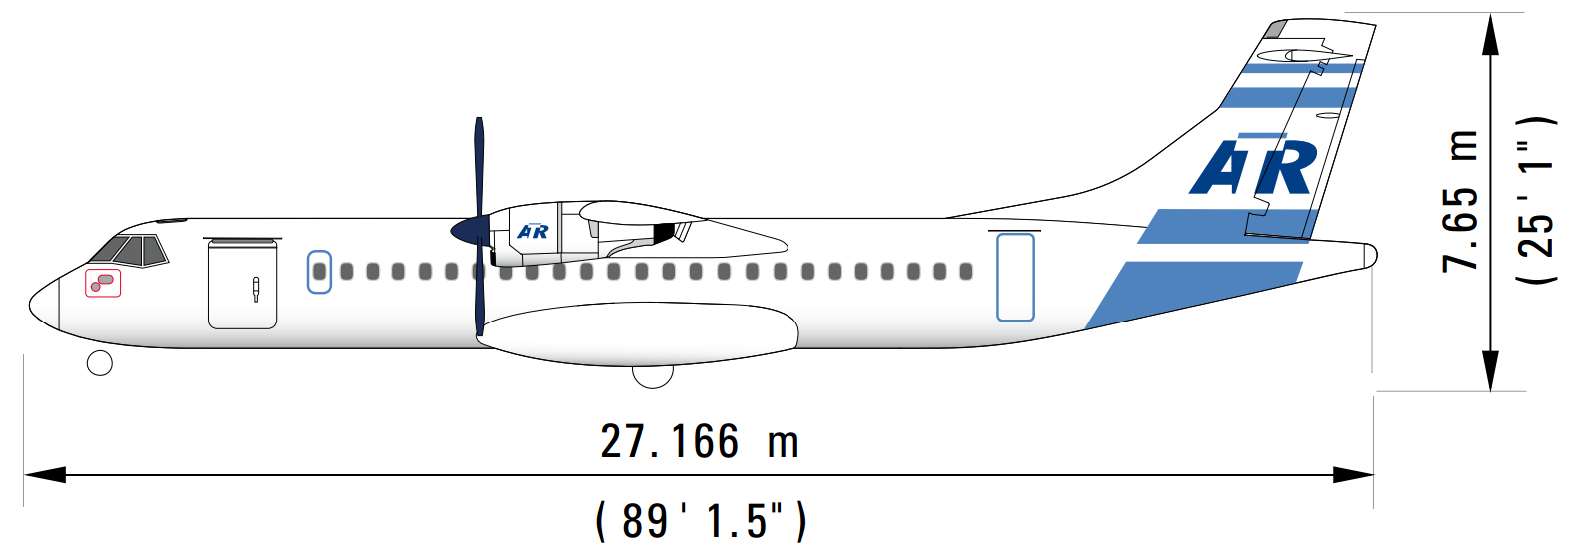
\includegraphics[height=4cm]{Immagini/atr72mod.jpg}} 
\caption{ATR 72. Side view.}
\end{figure}


The {\bfseries Boeing 747-100B} is a four-engined long-range widebody commercial jet airliner and cargo aircraft  produced by the American manufacturer Boeing Commercial Airplanes. It has a capacity of maximum 480 passengers in a partial double deck configuration. The Boeing 747 It is also known as Jumbo Jet. The basic B747-100 entered service with Pan American On January 15, 1970.\\
One of the reason to create the 747 was reductions in airfares with a consequent increase of passenger traffic\cite{wiki:boeing}. The original version of the 747 had two and a half times greater capacity than the Boeing 707, one of the common large commercial aircraft of the 1960s and it was the largest passenger carrier from 1970 until the introduction of Airbus A380.\cite{boeing:boeing}
The Boeing 747 had two aisle and four wing-mounted engines. The upper deck is its distinctive "hump" along the forward part of the aircraft. It provides space for a lounge or extra seating. The raised cockpit allows front loading of cargo on freight variants. \\
The 747-100B model was developed from the 747-100SR. This configuration had a typical 452 passengers and unlike the original 747-100, the 747-100B was offered with Pratt \& Whitney JT9D-7A, General Electric CF6-50, or Rolls-Royce RB211-524 turbofan engines.

\begin{figure}[H]
\centering
{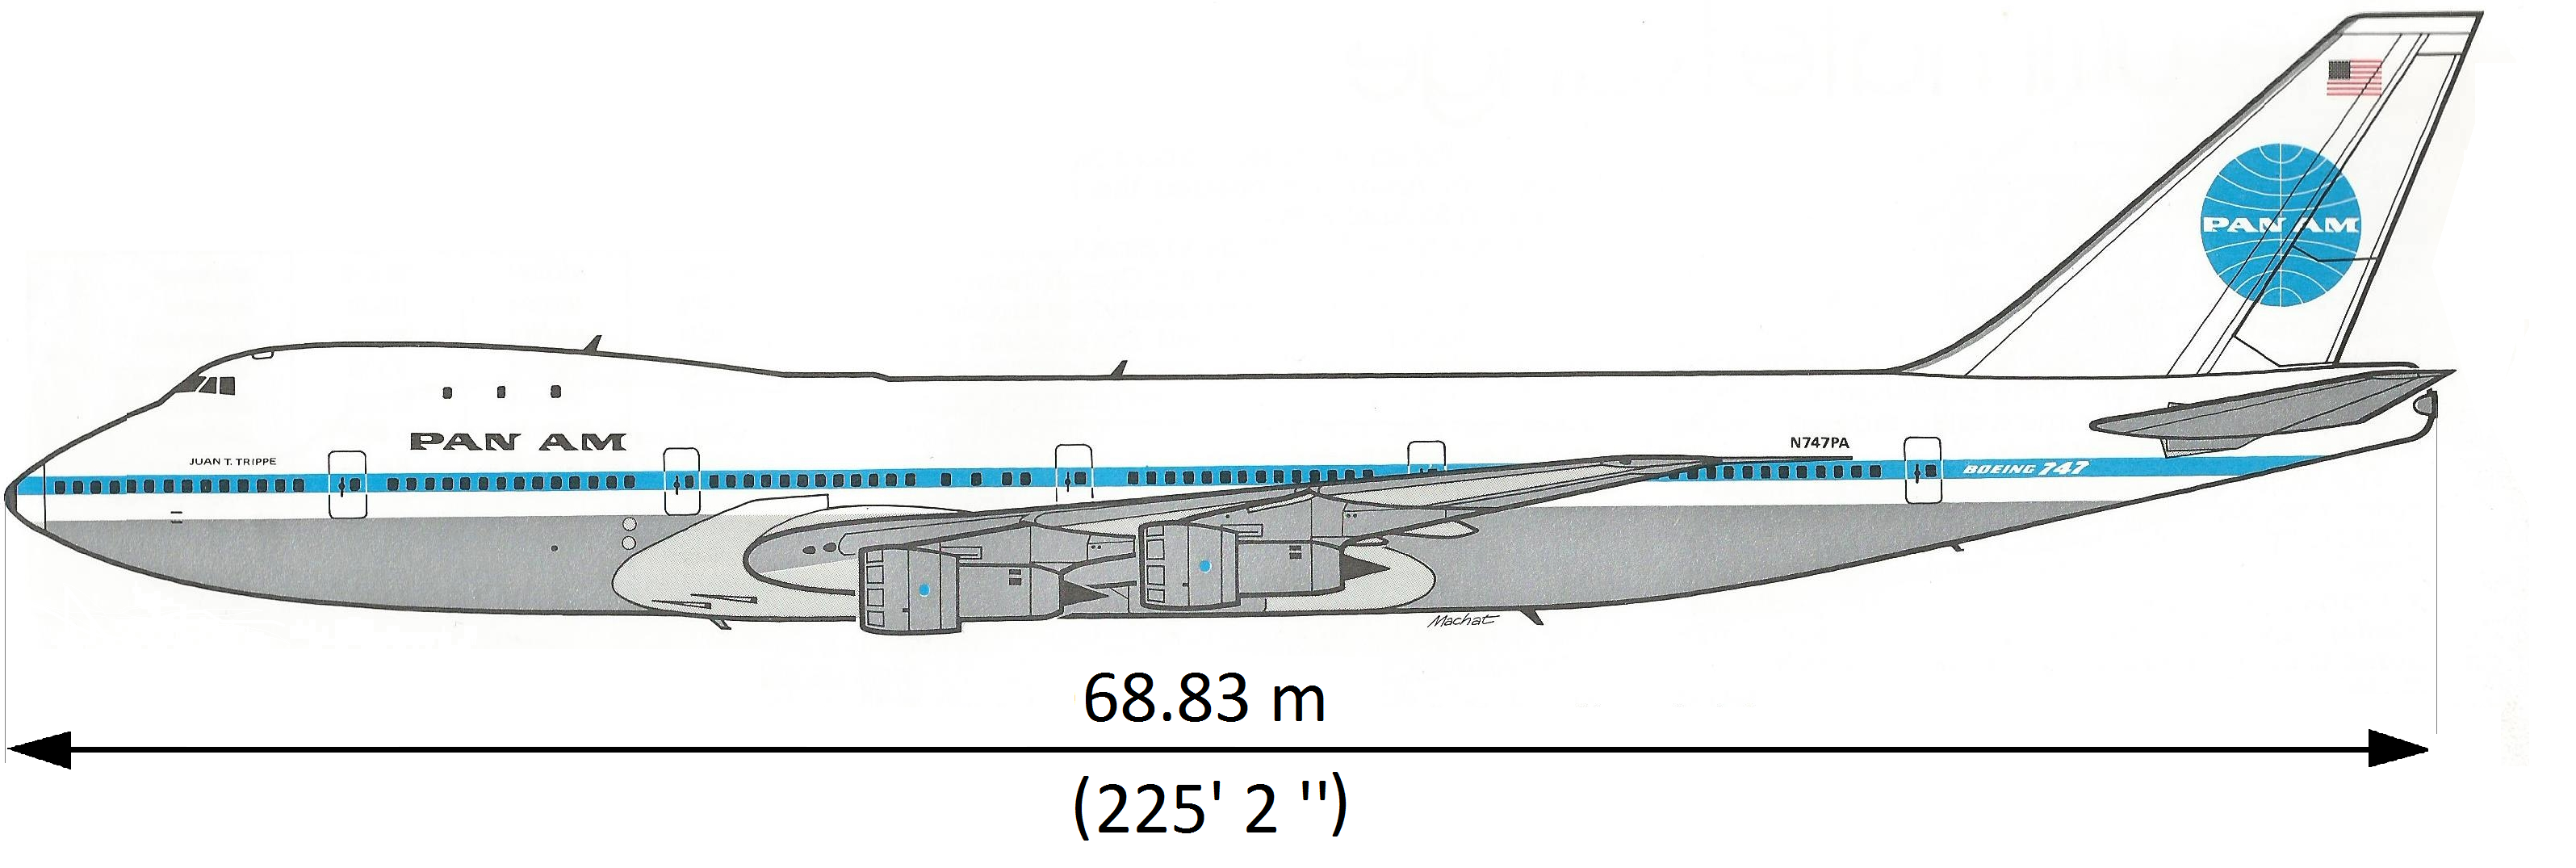
\includegraphics[height=4cm]{Immagini/boeing.jpg}} 
\caption{Boeing 747-100B. Side view.}
\end{figure}

\subsection {How is made a default Aircraft}
In order to define a Default Aircraft in a test class, and use it to check the functionalities of the application, it is necessary to follow some step. First of all it is necessary to initialize the working directory tree using the method \texttt{initWorkingDirectoryTree} of \texttt{MyConfiguration} class located in \texttt{JPADConfigs} package that initializes the working directory tree and fill the map of folders. 
This step is required in order to create the following default folders that are necessary for the right behavior of the code:

\begin{itemize}
\item Database directory
\item Input directory
\item Output directory
\end{itemize}

Using  \texttt{MyConfiguration} class it's possible to point at a specific folder, like the input or output directory, with the static method  \texttt{getDir}. This is a crucial step that must be execute at the beginning of every test.
To set the working directory with the useful folders, it's necessary to call the function \texttt{initWorkingDirectoryTree()} at the beginning of each test. The function creates all necessary folders. Morover the function has been overloaded and it can be even called with a variable number of arguments (\texttt{initWorkingDirectoryTree( String...str)}). These strings are the directory strings in \texttt{MyConfiguration} class.
After it is possible to create an \texttt{Aircraft} object choosing between ``ATR-72'' or ``B747-100B'' using the method \texttt{createDefaultAircraft} from \texttt{Aircraft} class. This method defines a new Aircraft object and invokes another Aircraft's methods that creates the component using deafult data. In the method \texttt{createDeafaultAircraft} there is a calling to the builder of \texttt{Aircraft} class that initializes the objects of the classes that perform calculations. At this step all the components of the aircraft are created. It is possible also to define new airfoil for the aircraft or change some data from the existing. \\
Afterwards it is necessary to set the operating conditions such as the number of Mach of analysis or altitude. Each default aircraft has a set of default condition but the user could to change them.\\
In order to manage all the aircraft related analysis it is necessary to define an object of the class  \texttt{ACAnalysisManager}. Similarly to the aircraft,  exist an analysis manager also for the wing that is an object of the  \texttt{LSAerodynamicAnalysis} class. \\
The next step is to define and assign the needed databases. This will be explained in detail in the next section.Finally it is possible to do analysis.

\noindent \\
\begin{lstlisting}[frame=rbl,caption={{\footnotesize Generation of default aircraft}},label= [style=\bfseries]{Listing}]
public static void main(String[] args) {

	// --------------------------------------------------------------
	// Define directory
	// --------------------------------------------------------------
	MyConfiguration.initWorkingDirectoryTree();


	// --------------------------------------------------------------
	// Generate default Aircraft
	// --------------------------------------------------------------
	Aircraft aircraft = Aircraft.createDefaultAircraft("B747-100B");
	LiftingSurface theWing = aircraft.get_wing();

	// Default operating conditions
	OperatingConditions theConditions = new OperatingConditions();		


	// --------------------------------------------------------------
	// Define an ACAnalysisManager Object
	// --------------------------------------------------------------
	ACAnalysisManager theAnalysis = new ACAnalysisManager(theConditions);
	theAnalysis.updateGeometry(aircraft);


	// --------------------------------------------------------------
	// Define an LSAerodynamicsManager Object
	// --------------------------------------------------------------
	LSAerodynamicsManager theLSAnalysis = new LSAerodynamicsManager ( 
			theConditions,
			theWing,
			aircraft
			);

		
	// --------------------------------------------------------------
	// Setup database(s)	
	// --------------------------------------------------------------
		
	theLSAnalysis.setDatabaseReaders(
			new Pair(DatabaseReaderEnum.AERODYNAMIC,
                          "Aerodynamic_Database_Ultimate.h5"),
			new Pair(DatabaseReaderEnum.HIGHLIFT,  
                          "HighLiftDatabase.h5")
			);

	
	// --------------------------------------------------------------
	// Do analysis
	// --------------------------------------------------------------
	theAnalysis.doAnalysis(aircraft, 
			AnalysisTypeEnum.AERODYNAMIC);
}
\end{lstlisting}

\begin{sidewaysfigure}

\centering
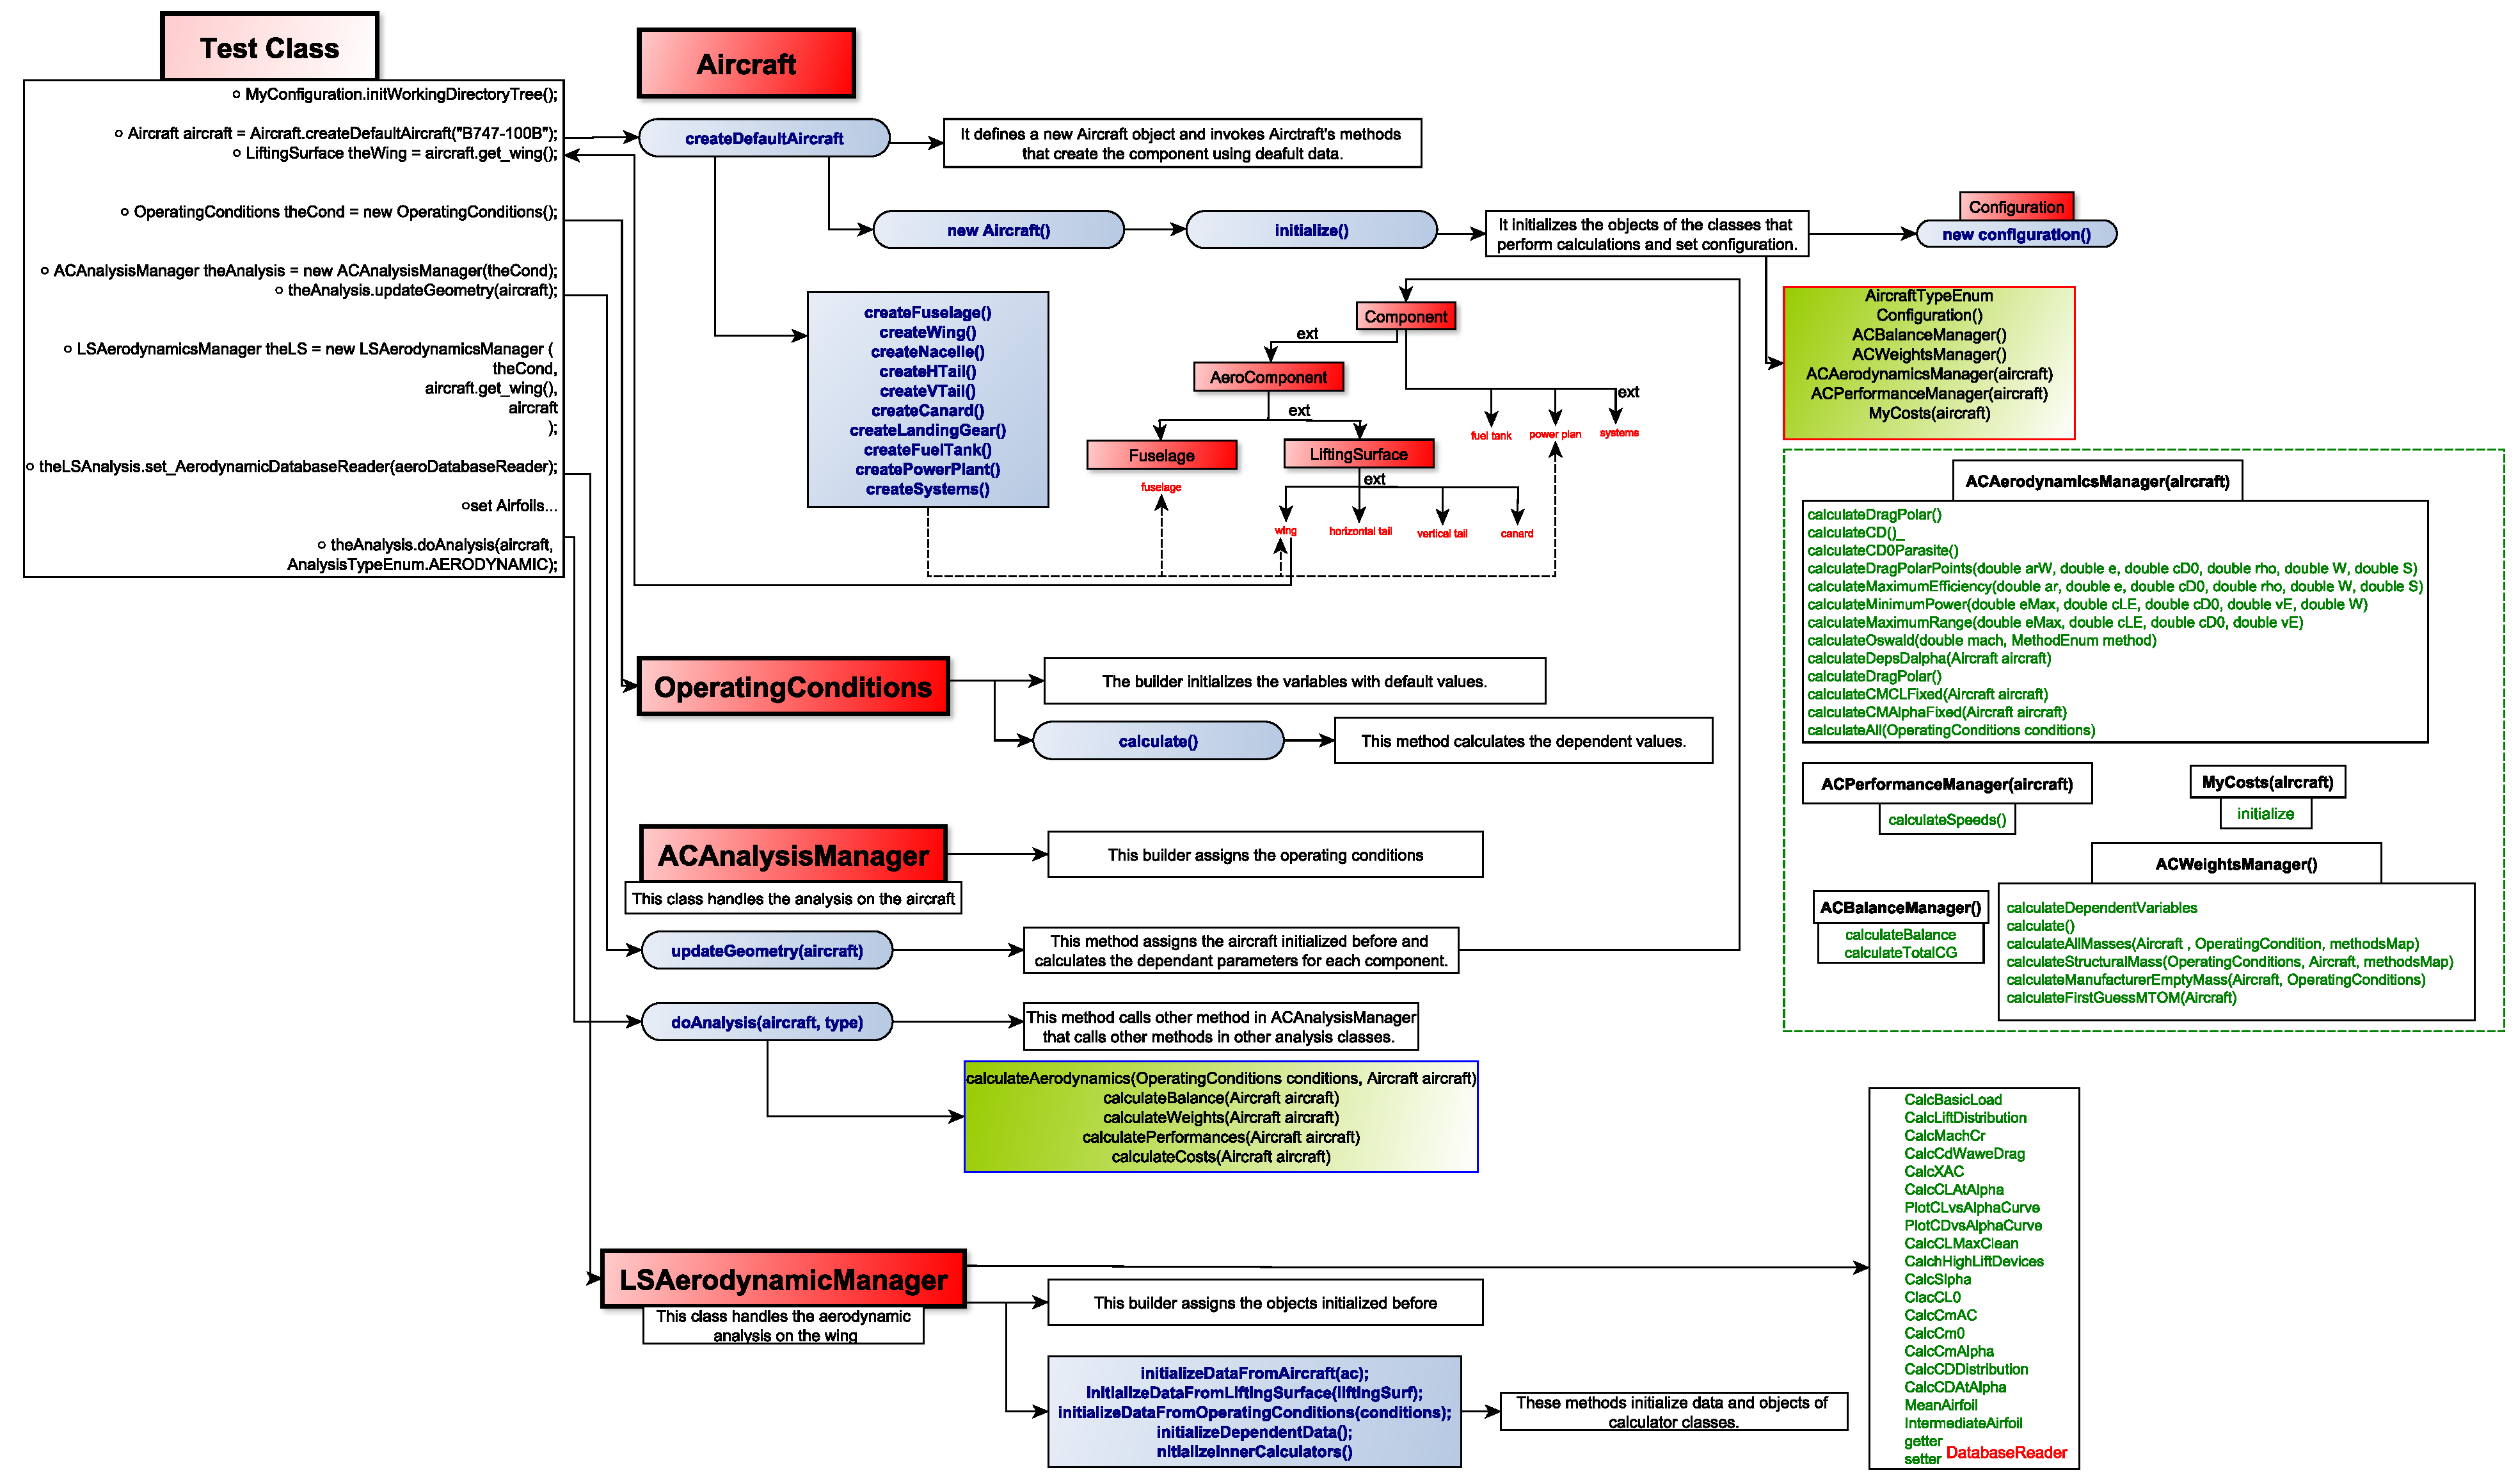
\includegraphics[width=24.6cm]{immagini/HowToCreateADefaultAircraftInJPAD3.pdf}
\caption{Flow chart of the creation of default Aircraft.}
\label{fig:schemauno}

\end{sidewaysfigure}

\subsection {How is made a default Wing}
Similary to the default aircraft it is possible to define a default wing. This is very useful if the user wants to make an analysis only on a wing. In this case it is necessary to define the origin of the \gls{acr:lrf} in \gls{acr:brf}
and the coordinates of the \gls{acr:cg}.\\
Contrary to the case of the aircraft, for an isolated wing there isn't necessary to define a fuselage in order to create a \texttt{Lifting Surface} object, but there is an overload of the builder that doesn't need a fuselage as input. In this case the exposed surface is calculated as the surface of the wing.

\noindent \\
\begin{lstlisting}[frame=rbl,caption={{\footnotesize Generation of an isolated Wing}},label= [style=\bfseries]{Listing}]
public static void main(String[] args) {

	// Assign all default folders
	MyConfiguration.initWorkingDirectoryTree();
	
	// -----------------------------------------------------------------------
	// Coordinates of LRF
	// -----------------------------------------------------------------------
	
	double xAw = 11.0; //meter 
	double yAw = 0.0;
	double zAw = 1.6;
	double iw = 0.0;
	
	// -----------------------------------------------------------------------
	// Generate default Wing
	// -----------------------------------------------------------------------
	
	LiftingSurface theWing = new LiftingSurface(
			"Wing", // name
			"Data from AC_ATR_72_REV05.pdf", 
			xAw, yAw, zAw, iw, 
			ComponentEnum.WING
			); 

	theWing.calculateGeometry();
	theWing.getGeometry().calculateAll();
	
	// -----------------------------------------------------------------------
	// Center of Gravity
	// -----------------------------------------------------------------------	
	
	double xCgLocal= 1.5; // meter 
	double yCgLocal= 0;
	double zCgLocal= 0;

	CenterOfGravity cg = new CenterOfGravity(
			Amount.valueOf(xCgLocal, SI.METER), // coordinates in LRF
			Amount.valueOf(yCgLocal, SI.METER),
			Amount.valueOf(zCgLocal, SI.METER),
			Amount.valueOf(xAw, SI.METER), // origin of LRF in BRF 
			Amount.valueOf(yAw, SI.METER),
			Amount.valueOf(zAw, SI.METER),
			Amount.valueOf(0.0, SI.METER),// origin of BRF
			Amount.valueOf(0.0, SI.METER),
			Amount.valueOf(0.0, SI.METER)
			);

	cg.calculateCGinBRF();
	theWing.set_cg(cg);
	theWing.set_aspectRatio(6.0);

	// Default operating conditions
	OperatingConditions theOperatingConditions = new OperatingConditions();		
	theOperatingConditions.set_alphaCurrent(Amount.valueOf(2.0, NonSI.DEGREE_ANGLE)

	// --------------------------------------------------------------
	// Define an LSAerodynamicsManager Object
	// --------------------------------------------------------------
	
	LSAerodynamicsManager theLSAnalysis = new LSAerodynamicsManager ( 
			theOperatingConditions,
			theWing
			);

	// --------------------------------------------------------------
	// Setup database(s)	
	// --------------------------------------------------------------
	
	theLSAnalysis.setDatabaseReaders(
			new Pair(DatabaseReaderEnum.AERODYNAMIC, 
					"Aerodynamic_Database_Ultimate.h5"),
			new Pair(DatabaseReaderEnum.HIGHLIFT, "HighLiftDatabase.h5")
			);
	
	// --------------------------------------------------------------
	// Assign Airfoil(s) ...	
	// --------------------------------------------------------------

	  // Define airfoilRoot...
	
	// --------------------------------------------------------------
	// Set Airofoil(s)	
	// --------------------------------------------------------------
	List<MyAirfoil> myAirfoilList = new ArrayList<MyAirfoil>();
	myAirfoilList.add(0, airfoilRoot);
	myAirfoilList.add(1, airfoilKink);
	myAirfoilList.add(2, airfoilTip);
	theWing.set_theAirfoilsList(myAirfoilList);
	theWing.updateAirfoilsGeometry(); 
	theLSAnalysis.initializeDependentData();

}
\end{lstlisting}

\section {Database in JPAD}

In JPAD it is possible to consult external databases in .h5 format. {\bfseries HDF 5} (Hierarchical Data Format Release 5) is a data file format designed by the {\itshape National Center for Supercomputing Applications} (NCSA) to assist users in the storage and manipulation of scientific data across different operating systems and machines.\\
To obtain the useful data in JPAD  interpolating functions are used . These functions can be of one, two or three dimensions and read data from graphics that have been digitize previously.\\
Starting from these digitalizations, databases in .h5 format are built.
Reading data from databases is entrusted to methods of classes in the \texttt{database} package.\\
In order to read these databases, and obtain the useful data, it is necessary to define an object of the database reading class and associate it with the object of analysis.\\
This is a crucial step to read correctly the external data. In fact JPAD allows to work with an aircraft object  or only with an isolated lifting surface object.  Aircraft is usually composed of a fuselage, lifting surfaces, nacelle and power plant.
Furthermore, \texttt{Aircraft} and \texttt{Wing} are associated with classes of calculation like \texttt{LSAerodynamicManager} or \texttt{ACAnalysisManager}. So it is necessary that these databases are also visible from these classes.\\
So because  both in aircraft and in wing there is a lifting surface object, databases relative to wing are associated to \texttt{LSAerodynamicManager}.

\subsection {Setup database}
Here the database path it's created and associated to object that interpolates the required data from the .h5 file using a \texttt{MyInterpolatingFunction} object. After this it's possible to access the double value of the interpolating function using the \texttt{standaloneutils} method called \texttt{value}. \\


%\begin{lstlisting}[frame=rbl,caption={{\footnotesize Setup database(s)}},label= [style=\bfseries]{Listing}]
%// --------------------------------------------------------------
%// Define database
%// --------------------------------------------------------------
%MyConfiguration.initWorkingDirectoryTree();
%
%// Setup database(s)	
%String databaseFolderPath = MyConfiguration.getDir(FoldersEnum.DATABASE_DIR);
%String databaseFileName = "Aerodynamic_Database_Ultimate.h5";
%AerodynamicDatabaseReader aeroDatabaseReader = 
%		new AerodynamicDatabaseReader(
%				databaseFolderPath, 
%				databaseFileName
%				);
%\end{lstlisting}

Now the procedure to assign the database is different if is used an Aircraft object or a Wing object.

\subsection {Assign database using an Aircraft object}
In order to assign correctly the database and associate it to all analysis management is necessary to practise the following order.
\begin{enumerate}
\item Define an Aircraft Object.\\This command associates to Aircraft an object that defines the aerodynamic. From the wing it is possible to obtain the Wing, that is a \texttt{LiftingSurface} object.
\item Define an \texttt{ACAnalysisManager} object.\\All the aircraft computations are managed by this class.
\item Define an \texttt{LSAerodynamicManager} object.\\ All the lifting surfaces computations are managed by this class.
\item Associate database to \texttt{LSAerodynamicManager}.
\item Eventually do analysis.
\end{enumerate}

\subsection {Assign database using a Wing object}
Using a Wing object it isn't neccessary to define a manager for Aircraft aerodynamic analysis. So the step to follow are the same of aircraft starting from the third.
\begin{enumerate}
\item Define an Wing Object.
\item Define an \texttt{LSAerodynamicManager} object.
\item Associate database to \texttt{LSAerodynamicManager}.
\end{enumerate}

The definition of a isolated Wing is explained in the relative section.

%\begin{lstlisting}[frame=rbl,caption={{\footnotesize Assign database using an Aircraft object}},label= [style=\bfseries]{Listing}]
%
%// --------------------------------------------------------------
%// Generate default Aircraft
%// --------------------------------------------------------------
%Aircraft aircraft = Aircraft.createDefaultAircraft("B747-100B");
%LiftingSurface theWing = aircraft.get_wing();
%		
%// Default operating conditions
%OperatingConditions theConditions = new OperatingConditions();		
%		
%		
%// --------------------------------------------------------------
%// Define an ACAnalysisManager Object
%// --------------------------------------------------------------
%ACAnalysisManager theAnalysis = new ACAnalysisManager(theConditions);
%theAnalysis.updateGeometry(aircraft);
%		
%		
%// --------------------------------------------------------------
%// Define an LSAerodynamicsManager Object
%// --------------------------------------------------------------
%LSAerodynamicsManager theLSAnalysis = new LSAerodynamicsManager ( 
%		theConditions,
%		theWing,
%		aircraft
%		);
%		
%		
%// --------------------------------------------------------------
%// Associate database to LSAerodynamicManager
%// --------------------------------------------------------------
%theLSAnalysis.set_AerodynamicDatabaseReader(aeroDatabaseReader);
%
%		
%// --------------------------------------------------------------
%// Do analysis
%// --------------------------------------------------------------
%theAnalysis.doAnalysis(aircraft, 
%		AnalysisTypeEnum.AERODYNAMIC);
%\end{lstlisting}

\noindent \\
\begin{lstlisting}[frame=rbl,caption={{\footnotesize Assign database using an Aircraft object}},label= [style=\bfseries]{Listing}]
		
	// --------------------------------------------------------------
	// Setup database(s)	
	// --------------------------------------------------------------
		
	theLSAnalysis.setDatabaseReaders(
			new Pair(DatabaseReaderEnum.AERODYNAMIC,
                          "Aerodynamic_Database_Ultimate.h5"),
			new Pair(DatabaseReaderEnum.HIGHLIFT,  
                          "HighLiftDatabase.h5")
			);

\end{lstlisting}
The databases are assigned to \texttt{LSAerodynamic} using a method of this class. This method accept as input a variable number of \texttt{Pair} objects.Using \texttt{Pair} objects it is possible to assign, for each database, both name and type. 

\noindent \\
\begin{lstlisting}[frame=rbl,caption={{\footnotesize \texttt{setDatabaseReaders} method}},label= [style=\bfseries]{Listing}]

public void setDatabaseReaders(Pair... args) {
	String databaseFolderPath = MyConfiguration.getDir(FoldersEnum.DATABASE_DIR);
	
	for (Pair a : args) {
		DatabaseReaderEnum key = (DatabaseReaderEnum)a.getKey(); 
		String databaseFileName = (String)a.getValue();
		
		switch (key) {
			case AERODYNAMIC:
				_aerodynamicDatabaseReader = 
				new AerodynamicDatabaseReader(
						databaseFolderPath,
						databaseFileName); 
				listDatabaseReaders.add(_aerodynamicDatabaseReader);
				break;
				
			case HIGHLIFT:
				_highLiftDatabaseReader = 
				new HighLiftDatabaseReader(
						databaseFolderPath, 
						databaseFileName); 
				listDatabaseReaders.add(_highLiftDatabaseReader);
			break;	
			
		}
\end{lstlisting}


\subsection {Developer's guide}

In order to execute some analysis in JPAD it is necessary, first of all, to define an analysis object in the Test class. The method \texttt{createDefaultAircraft} creates a new aircraft and the object that composes it. This method also populates the data of aircraft with default value corresponding to ATR-72 or Boieng 747\_100B. Moreover the method \texttt{createDefaultAircraft} calls another method in \texttt{Aircraft} class: \texttt{initialize} that initializes the objects of the classes that perform calculations. \\
The purpose of this structure is to have only a way to assign the databases at an aircraft. Inasmuch as the wing is always present, the chosen strategy is to assign the database to the aerodynamic manager of the wing.\\
In order to bring to use the database also for the aircraft calculation, it is assigned at the aerodynamic manager of the aircraft in the method called \texttt{doAnalysis}.\\
At the same time \texttt{LSAerodynamicManager} sets itself as aerodynamic in the wing object. \\
So it is possible to call the database using equally the following codes: 
\begin{itemize}
\item \texttt{theWingObject.getAerodynamics.get\_Database;}
\item \texttt{theAircraftObject.get\_theAerodynamic.get\_Database;}
\item \texttt{theLSManagerObject.get\_Database;}
\item \texttt{theACManagerObject.get\_Database;}
\end{itemize}

\begin{sidewaysfigure}

\centering
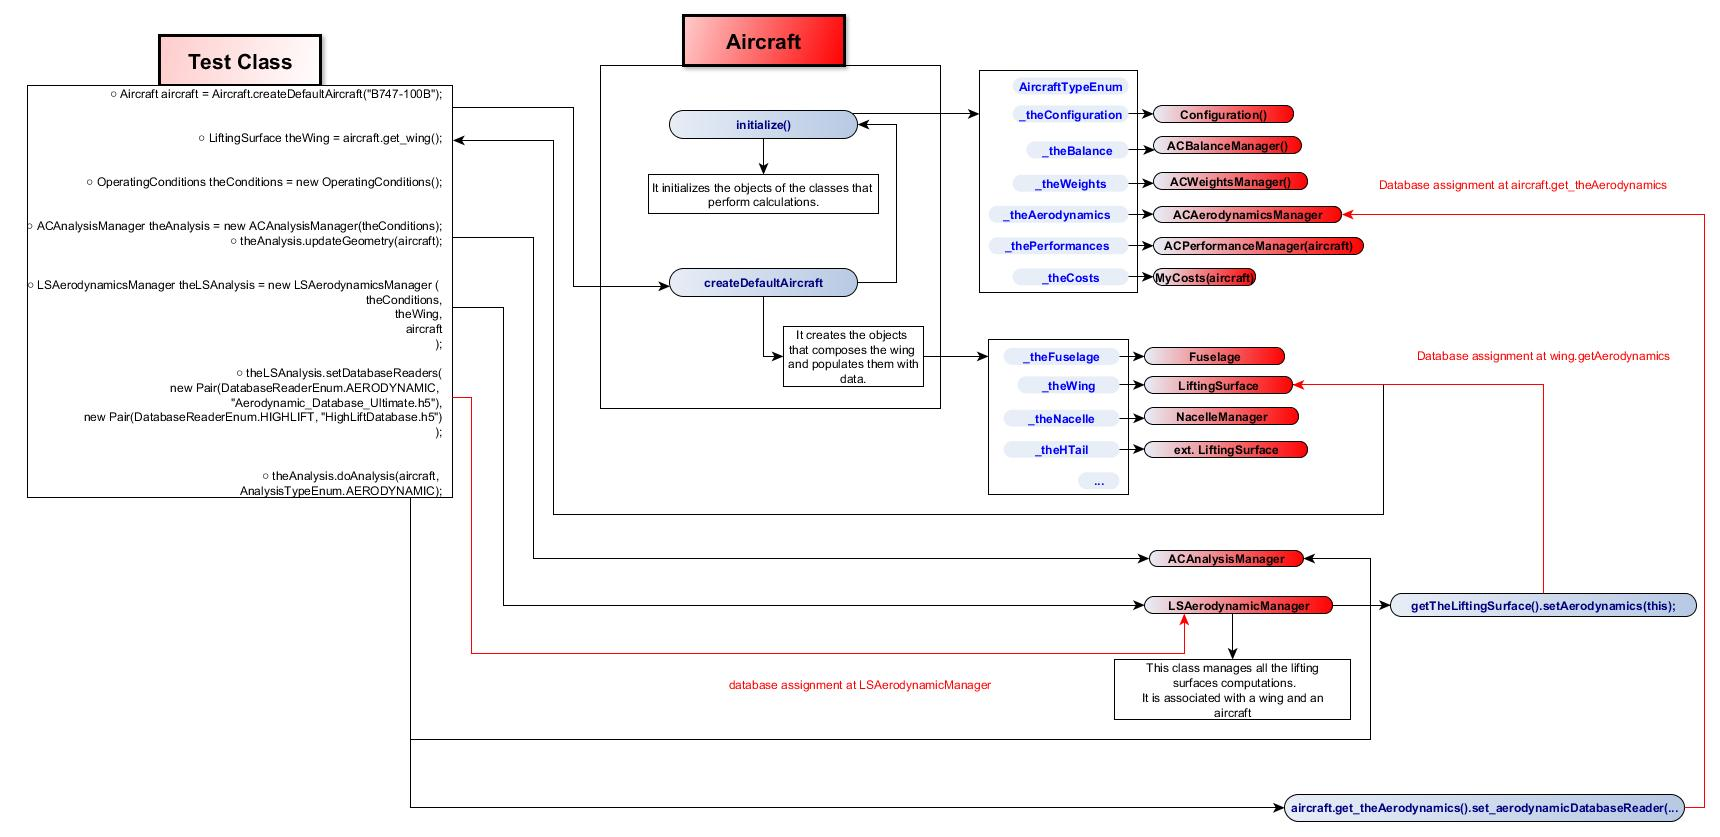
\includegraphics[width=23cm]{immagini/HowToAssignDatabase.jpg}
\caption{Flow chart of database assignment.}
\label{fig:schemauno}

\end{sidewaysfigure}